\PassOptionsToPackage{unicode=true}{hyperref} % options for packages loaded elsewhere
\PassOptionsToPackage{hyphens}{url}
\documentclass[11pt,dvipsnames,ignorenonframetext,aspectratio=169]{beamer}
\IfFileExists{pgfpages.sty}{\usepackage{pgfpages}}{}
\setbeamertemplate{caption}[numbered]
\setbeamertemplate{caption label separator}{: }
\setbeamercolor{caption name}{fg=normal text.fg}
\beamertemplatenavigationsymbolsempty
\usepackage{lmodern}
\usepackage{amssymb,amsmath}
\usepackage{ifxetex,ifluatex}
\usepackage{fixltx2e} % provides \textsubscript
\ifnum 0\ifxetex 1\fi\ifluatex 1\fi=0 % if pdftex
  \usepackage[T1]{fontenc}
  \usepackage[utf8]{inputenc}
\else % if luatex or xelatex
  \ifxetex
    \usepackage{mathspec}
  \else
    \usepackage{fontspec}
\fi
\defaultfontfeatures{Ligatures=TeX,Scale=MatchLowercase}







\fi

  \usetheme[]{monash}

  \usecolortheme{monashwhite}


% A default size of 24 is set in beamerthememonash.sty

% Title page
\setbeamertemplate{title page}
{\placefig{-0.01}{-0.01}{width=1.01\paperwidth,height=1.01\paperheight}{zymoseptoria\_fungus\_growing\_on\_wheat.jpg}
\begin{textblock}{7.5}(1,2.8)\usebeamerfont{title}
{\color{white}\raggedright\par\inserttitle}
\end{textblock}
\begin{textblock}{7.5}(1,7)
{\color{white}\raggedright{\insertauthor}\mbox{}\\[0.2cm]
\insertdate}
\end{textblock}}


  \useinnertheme{rounded}

  \useoutertheme{smoothtree}

% use upquote if available, for straight quotes in verbatim environments
\IfFileExists{upquote.sty}{\usepackage{upquote}}{}
% use microtype if available
\IfFileExists{microtype.sty}{%
  \usepackage{microtype}
  \UseMicrotypeSet[protrusion]{basicmath} % disable protrusion for tt fonts
}{}


\newif\ifbibliography
  \usepackage[round]{natbib}
  \bibliographystyle{plainnat}


\hypersetup{
      pdftitle={Sources and Test of Resistance},
            colorlinks=true,
    linkcolor=red,
    citecolor=Blue,
    urlcolor=lightgrayd,
    breaklinks=true}
%\urlstyle{same}  % Use monospace font for urls







% Prevent slide breaks in the middle of a paragraph:
\widowpenalties 1 10000
\raggedbottom

  \AtBeginPart{
    \let\insertpartnumber\relax
    \let\partname\relax
    \frame{\partpage}
  }
  \AtBeginSection{
    \ifbibliography
    \else
      \let\insertsectionnumber\relax
      \let\sectionname\relax
      \frame{\sectionpage}
    \fi
  }
  \AtBeginSubsection{
    \let\insertsubsectionnumber\relax
    \let\subsectionname\relax
    \frame{\subsectionpage}
  }



\setlength{\parindent}{0pt}
\setlength{\parskip}{6pt plus 2pt minus 1pt}
\setlength{\emergencystretch}{3em}  % prevent overfull lines
\providecommand{\tightlist}{%
  \setlength{\itemsep}{0pt}\setlength{\parskip}{0pt}}

  \setcounter{secnumdepth}{0}


%% Monash overrides
\AtBeginSection[]{
   \frame<beamer>{
   \frametitle{Outline}\vspace*{0.2cm}
   
   \tableofcontents[currentsection,hideallsubsections]
  }}

% Redefine shaded environment if it exists (to ensure text is black)
\ifcsname Shaded\endcsname
  \definecolor{shadecolor}{RGB}{225,225,225}
  \renewenvironment{Shaded}{\color{black}\begin{snugshade}\color{black}}{\end{snugshade}}
\fi
%%


  \usepackage{setspace}
  \usepackage{wasysym}
  % \usepackage{footnote} % don't use this this breaks all
  \usepackage{fontenc}
  \usepackage{fontawesome}
  \usepackage{booktabs,siunitx}
  \usepackage{longtable}
  \usepackage{array}
  \usepackage{multirow}
  \usepackage{wrapfig}
  \usepackage{float}
  \usepackage{colortbl}
  \usepackage{pdflscape}
  \usepackage{tabu}
  \usepackage{threeparttable}
  \usepackage{threeparttablex}
  \usepackage[normalem]{ulem}
  \usepackage{makecell}
  \usepackage{xcolor}
  \usepackage{tikz} % required for image opacity change
  \usepackage[absolute,overlay]{textpos} % for text formatting
  \usepackage{chemfig}
  \usepackage[skip=0.333\baselineskip]{caption}
  % \newcommand*{\AlignChar}[1]{\makebox[1ex][c]{\ensuremath{\scriptstyle#1}}}%
  \usepackage{siunitx}

  % this font option is amenable for beamer
  \setbeamerfont{caption}{size=\tiny}
  \singlespacing
  \definecolor{lightgrayd}{gray}{0.95}
  \definecolor{skyblued}{rgb}{0.65, 0.6, 0.94}
  \definecolor{oranged}{RGB}{245, 145, 200}

  % % better to insert it into template itself
  % \newlength{\cslhangindent}
  % \setlength{\cslhangindent}{1.5em}
  % \newenvironment{cslreferences}%
  %   {\setlength{\parindent}{0pt}%
  %   \everypar{\setlength{\hangindent}{\cslhangindent}}\ignorespaces}%
  %   {\par}

  \usepackage[caption=false]{subfig}

  \newcommand{\bcolumns}{\begin{columns}[T, onlytextwidth]}
  \newcommand{\ecolumns}{\end{columns}}

  \newcommand{\bdescription}{\begin{description}}
  \newcommand{\edescription}{\end{description}}

  \newcommand{\bitemize}{\begin{itemize}}
  \newcommand{\eitemize}{\end{itemize}}
  \AtBeginSubsection{}

  \title[]{Sources and Test of Resistance}


  \author[
        Deependra Dhakal\\
Assistant Professor\\
Agriculture and Forestry University\\
\textit{ddhakal.rookie@gmail.com}\\
\url{https://rookie.rbind.io}
    ]{Deependra Dhakal\\
Assistant Professor\\
Agriculture and Forestry University\\
\textit{ddhakal.rookie@gmail.com}\\
\url{https://rookie.rbind.io}}


\date[
      
  ]{
    }

\begin{document}

% Hide progress bar and footline on titlepage
  \begin{frame}[plain]
  \titlepage
  \end{frame}


   \frame<beamer>{
   \frametitle{Outline}\vspace*{0.2cm}
   
   \tableofcontents[hideallsubsections]
  }

\hypertarget{non-host-mutations-genetic-modification}{%
\section{Non host, mutations, genetic
modification}\label{non-host-mutations-genetic-modification}}

\begin{frame}{Sources of resistance}
\protect\hypertarget{sources-of-resistance}{}
\begin{enumerate}
\tightlist
\item
  Commercial cultivars
\end{enumerate}

\begin{itemize}
\tightlist
\item
  Cultivars which are currently in cultivation or are available already
  somewhere
\item
  Advantage: rapidly development of new commercially useful cultivar,
  without many undesirable characters
\item
  With allogamous crops this is a more obvious possibility than for
  autogamous crops; i.e., in pea, an unsuspected resistance against
  \textit{Fusarium oxysporum} f.~sp. \textit{pisi} was found in some
  cultivars
\item
  Using exotic cultivar as source of resistance may be
  counterproductive, as

  \begin{itemize}
  \footnotesize
  \item introgression of the resistance may demand more efforts,
  \item exotic genotypes often have inadequate day length requirements
  \item possess properties that are not appreciated by local consumers
  \end{itemize}
\item
  When a common source of resistance is used in multiple occasions, one
  or few of the same genes will occur in high frequency in acerage of
  the crop

  \begin{itemize}
  \footnotesize
  \item in the events of breakdown of the resistance, all cultivars with that resistance will become vulnerable
  \end{itemize}
\end{itemize}
\end{frame}

\begin{frame}{Crop varieties of Nepal with notable characters}
\protect\hypertarget{crop-varieties-of-nepal-with-notable-characters}{}
\bcolumns
\column{0.5\textwidth}
\begin{table}
\centering\begingroup\fontsize{4}{6}\selectfont

\begin{tabular}{>{\raggedright\arraybackslash}p{5em}>{\raggedright\arraybackslash}p{10em}>{\raggedright\arraybackslash}p{32em}}
\toprule
Crop & Characteristic & Varieties\\
\midrule
 & Drought tolerance & Sukkha dhan-1, Sukkha dhan-2, Sukkha dhan-3, Sukkha dhan-4, Sukkha dhan-5, Sukkha dhan-6, Tarahara, Hardinath-2\\
\cmidrule{2-3}
 & Submergence tolerance & Swarna sub-1, Samba masuli sub-1, Ciherang sub-1\\
\cmidrule{2-3}
 & Drought and submergence tolerance & Bahuguni-1, Bahuguni-2, Sukkha dhan-6\\
\cmidrule{2-3}
 & Cold tolerance & Lekali dhan-1, Lekali dhan-3, Chandannath-3\\
\cmidrule{2-3}
 & Aromatic & Sunaulo sugandha, Sugandhit dhan-1, Lalkha basmati\\
\cmidrule{2-3}
\multirow{-6}{*}{\raggedright\arraybackslash Rice} & Hybrid & Hardinath hybrid dhan-1, Hardinath hybrid dhan-3\\
\cmidrule{1-3}
 & Drought tolerance & Deuti\\
\cmidrule{2-3}
 & High protein content & Poshilo makai-1, Poshil makai-2\\
\cmidrule{2-3}
 & Hybrid & Khumal hybrid-2, Rampur hybrid-1\\
\cmidrule{2-3}
 & Quick maturing & Arun-2, Arun-3, Arun-4 (90 days), Arun 6 (80 days)\\
\cmidrule{2-3}
\multirow{-5}{*}{\raggedright\arraybackslash Maize} & Dhwase theglo rog tolerance & Manakamana-3, Ganesh-1, Sheetal, Deuti, Khumal hybrid-2\\
\bottomrule
\end{tabular}
\endgroup{}
\end{table}

\column{0.5\textwidth}

\begin{table}
\centering\begingroup\fontsize{4}{6}\selectfont

\begin{tabular}{>{\raggedright\arraybackslash}p{5em}>{\raggedright\arraybackslash}p{8em}>{\raggedright\arraybackslash}p{26em}}
\toprule
Crop & Characteristic & Varieties\\
\midrule
 & UG-99 tolerant & Bijay, Danfe, Tilottama, Swargadwari, Banganga\\
\cmidrule{2-3}
 & Heat tolerance (late) & Gautam, Bijay\\
\cmidrule{2-3}
 & Leaf blight & Bijay, Danfe, Tilottama, Gautam\\
\cmidrule{2-3}
 & Rust (Black, brown, yellow) tolerant & Munal, Chyakhura\\
\cmidrule{2-3}
\multirow{-5}{*}{\raggedright\arraybackslash Wheat} & Durum & Khajura durum-1, Khajura durum-2\\
\cmidrule{1-3}
Rapeseed/mustard & High yielding and drought tolerance & Lumle tori-1\\
\cmidrule{1-3}
 & Useful for making chips & Khumal bikash, Khumal ujjwal, Khumal seto-1\\
\cmidrule{2-3}
\multirow{-2}{*}{\raggedright\arraybackslash Potato} & Blight resistant & Janakdev, Khumal bikash, Khumal ujjwal, Khumal rato-2, Khumal seto-1, Khumal upahar\\
\bottomrule
\end{tabular}
\endgroup{}
\end{table}

\ecolumns
\end{frame}

\begin{frame}{}
\protect\hypertarget{section}{}
\small

\begin{enumerate}
\setcounter{enumi}{1}
\tightlist
\item
  Other varieties
\end{enumerate}

\begin{itemize}
\tightlist
\item
  Resistance to a certain natural enemy may occur in one variety but not
  in other
\item
  Some variety serve as useful sources of resistance
\item
  Perennial kale ( \emph{Brassica oleracea} var. \emph{ramosa}) may be
  more resistant against club root ( \emph{Plasmodiophora brassicae})
  than for instance cabbage (\emph{B. oleracea} var. \emph{capitata})
\end{itemize}

\begin{enumerate}
\setcounter{enumi}{2}
\tightlist
\item
  Landraces
\end{enumerate}

\begin{itemize}
\tightlist
\item
  Often contain significant genetic diversity and have been cultivated
  for a long period of time, usually under rather primitive cultural
  practices
\item
  When the pathogenic outbreak/infestation due to natural enemy occured
  in the regions of the origin of the landrace, natural selection for
  resistance may have taken place.
\item
  In a landrace collection panel of barley from Syria and Jordan,
  diversity of resistance (absolute and partial resistance as well as
  high susceptibility) was observed for each pathogen both between
  populations of different collection sites as well as between head
  progenies within collection sites\citep{van1989diversity}.
\end{itemize}
\end{frame}

\begin{frame}{}
\protect\hypertarget{section-1}{}
\begin{enumerate}
\setcounter{enumi}{3}
\tightlist
\item
  Wild progenitor species
\end{enumerate}

\begin{itemize}
\tightlist
\item
  Belongs to the same botanical species as the crop and can be crossed
  readily without problems of poor chromosome pairing or sterility
\item
  Usually have a huge diversity for resistance
\item
  Natural enemy and host species usually have occured side by side for
  ages and have co-evolved, leading to the variation in the host.
\end{itemize}

\begin{enumerate}
\setcounter{enumi}{4}
\tightlist
\item
  Related species
\end{enumerate}

\begin{itemize}
\tightlist
\item
  Can be exploited when the resistance is not available in the botanical
  species itself

  \begin{itemize}
  \tightlist
  \item
    Potato resistance against bacterium \emph{Pseudomonas solanacearum}
    was found in \emph{S. phureja}
  \item
    Genera of closely related ancestory such as \emph{O. sativa} with
    \emph{O. rufipogon} and \emph{O. nivara} can be exploited as
    potential source of resistance (Sheath blight casused by
    \emph{Rhizoctonia solani}, for exmaple) more easily than other (such
    as \emph{O. officinalis}) which are distantly related.
  \end{itemize}
\end{itemize}
\end{frame}

\begin{frame}{}
\protect\hypertarget{section-2}{}
\bcolumns
\column{0.3\textwidth}
\footnotesize

\begin{enumerate}
\setcounter{enumi}{5}
\tightlist
\item
  Related genera
\end{enumerate}

\begin{itemize}
\tightlist
\item
  Is a long and difficult process and resistance obtained often appear
  to be not more durable than the resistance found in the cultiaved
  species
\item
  A chromosome segment from rye ( \emph{Secale cereale}) has been
  introduced into wheat that bear the genes conferring resistance to
  wheat yellow rust, leaf rust and stem rust
\end{itemize}

\column{0.7\textwidth}
\renewcommand{\arraystretch}{0.8}

\begin{table}

\caption{\label{tab:wild-related-species-disease-gene-transfer}Wild/related species of different crops with potential use, for bearing resistance gene, as source material in varietal breeding}
\centering
\fontsize{5}{7}\selectfont
\begin{tabular}[t]{>{\raggedright\arraybackslash}p{5em}>{\raggedright\arraybackslash}p{20em}>{\raggedright\arraybackslash}p{28em}}
\toprule
Crop & Disease/pathogen & Wild/related species\\
\midrule
 & Grassy stunt virus & Oryza nivara\\
\cmidrule{2-3}
\multirow{-2}{*}{\raggedright\arraybackslash Rice} & Stem rot (Sclerotium oryzae sativae) & O. rufipogon, O. nivara\\
\cmidrule{1-3}
 & Stem rust (Puccinia graminis f.sp. Tritici) & Triticum boeticum, T. monococcum, T. durum, Agropyron elongatum\\
\cmidrule{2-3}
 & Brown rust (P. recondita f. sp. Tritici) & Agropyron elongatum, A. monococcum\\
\cmidrule{2-3}
\multirow{-3}{*}{\raggedright\arraybackslash Wheat} & Yellow rust (P. striiformis) & Aegilops comosa\\
\cmidrule{1-3}
Barley & Powdery mildew (Erysiphe graminis f. sp. Hordei) & Hordeum spontaneum, H. bulbosum\\
\cmidrule{1-3}
Grapes & Downy mildew (Plasmopara viticola) & Vitis unifera var. sylvestris\\
\cmidrule{1-3}
 & Wilt (Fusarium oxysporum f. sp. Lycopersici) & Lycopersicum pimpinellifolium\\
\cmidrule{2-3}
\multirow{-2}{*}{\raggedright\arraybackslash Tomato} & Blight (Septoria lycopersici) & L. hirsutum\\
\cmidrule{1-3}
 & Late blight (Phytophthora infestans) & Solanum demissum, S. bulbocastanum\\
\cmidrule{2-3}
 & Charcol rot (Marophomina phaseolina) & S. chacoense\\
\cmidrule{2-3}
\multirow{-3}{*}{\raggedright\arraybackslash Potato} & Virus X & S. cartilobum\\
\bottomrule
\end{tabular}
\end{table}

\ecolumns
\end{frame}

\begin{frame}{Difficulties with use of diverse source of germplasm}
\protect\hypertarget{difficulties-with-use-of-diverse-source-of-germplasm}{}
\begin{itemize}
\tightlist
\item
  Using exotic or landrace cultivar, including unadapted varieties, and
  wild progenitors as source require frequent back-crossing and
  selection to get rid of numerous undesirable traits of the donor
  parent.

  \begin{itemize}
  \tightlist
  \item
    breeding for late blight resistance in potato is challenging since
    the resistance is linked to late maturity and photoperiod
    sensitivity
  \end{itemize}
\item
  Even related species or adapted varieties may present complications
  due to

  \begin{itemize}
  \tightlist
  \item
    limited crossability
  \item
    asynchrony
  \item
    hybrid sterility and poor seed recovery
  \item
    poor exchange of chromosome segments
  \end{itemize}
\item
  Althewhile, it is nearly impossible to eliminate all the characters of
  the donor genotype.
\end{itemize}
\end{frame}

\begin{frame}{Non host species as source of resistance}
\protect\hypertarget{non-host-species-as-source-of-resistance}{}
\bcolumns
\column{0.70\textwidth}
\small

\begin{itemize}
\tightlist
\item
  Most plants are non-host to most pathogens
\item
  Two plant species that are sufficiently closely related to be crossed,
  but still sufficiently unrelated to differ in host status to the
  target population
\item
  Barley is typically susceptible to \emph{P. hordei}, to which wheat is
  a non-host.

  \begin{itemize}
  \tightlist
  \item
    In wheat cultivar Duri, the majority of the colonies of \emph{P.
    hordei} produced no haustoria. The non-host resistance mechanism
    involves necrosis of mesophyll cells and blocking of the fungus
    before the haustorium development (more than 50\% colonies in the
    studies could not form haustorium), possibly becuase of a failing
    recognition reaction at the interface of the Haustorial Mother Cell
    (HMC) and the plant cell wall.
  \end{itemize}
\end{itemize}

\column{0.3\textwidth}

\begin{figure}
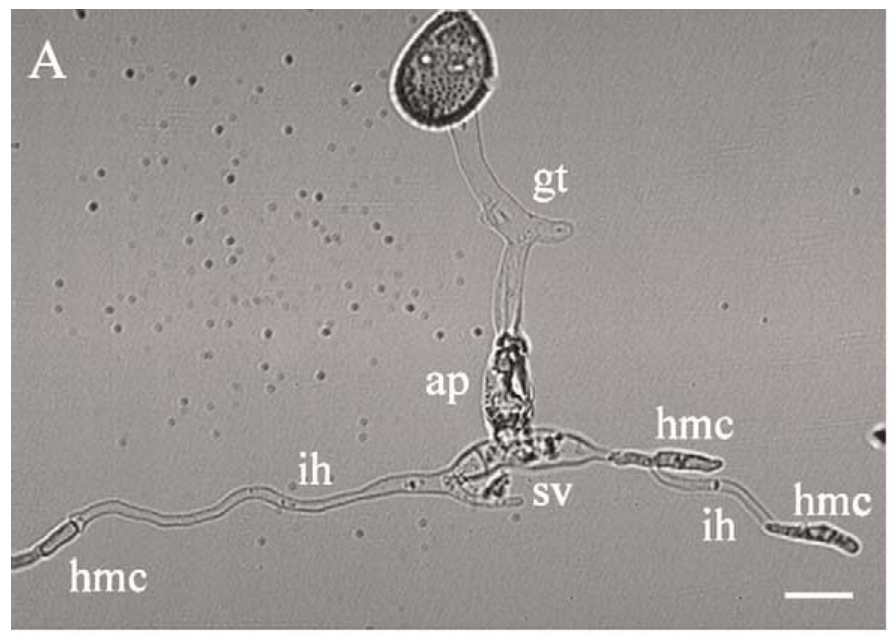
\includegraphics[width=0.98\linewidth]{../images/haustorial_mother_cell} \caption{In vitro differentiation of infection structures including haustorial mother cells by the wheat stem rust fungi \textit{Puccinia graminis} f. sp. \textit{tritici} after application of a mild heat shock (2h, \SI{30}{\celsius}) and trans-2-hexen-1-ol (0.5mM) in a humid atmosphere. Fully differentiated germlings using bright field optics is being shown (gt, germ tube; ap, appresorium; sv, substomatal vesicle; ih, infection hypha; hmc, haustorial mother cell) (bar: \SI{15}{\micro\meter}); Source: \cite{wietholter2003vitro}}\label{fig:haustorial-mother-cell}
\end{figure}

\ecolumns
\end{frame}

\begin{frame}{Mutation breeding of resistance}
\protect\hypertarget{mutation-breeding-of-resistance}{}
\begin{itemize}
\tightlist
\item
  Alternatively, mutation is a viable strategy for breeding for
  resistance if

  \begin{itemize}
  \tightlist
  \item
    no other known sources of resistance are available against target
    pathogen, or if existing resistance types are ephemeral
  \item
    resistance, although known to exist, is not a very difficult to
    introduce, like in vegetatively propagated crops as sugarcane and
    potato.
  \end{itemize}
\item
  A susceptible cultivar may be changed into a resistant one with
  mutation breeding, given a suitable procedure for induction and
  screening are practiced
\item
  Usually side effects of the mutagenic treatments do occur, although
  much of the agronomic traits are unaffected

  \begin{itemize}
  \tightlist
  \item
    in barley, resistance against powdery mildew ( \emph{Erysiphe
    graminis}) has been induced by mutagenesis repeatedly and in several
    cultivars.
  \end{itemize}
\item
  Resistance obtained by mutagenesis are not necessarily stable
  (possibly epigenetic inheritance)
\item
  Huge number of plants/lines should be tested because of low frequency
  of recovery of desired mutants for resistance
\end{itemize}
\end{frame}

\begin{frame}{Genetic modification}
\protect\hypertarget{genetic-modification}{}
\begin{itemize}
\tightlist
\item
  Refer to \citet{pavan2008map} for how to clone a resistance gene
\item
  For a discussion of transformation techniques, refer to Lecture notes
  of Introductory Biotechnology.
\end{itemize}
\end{frame}

\hypertarget{test-of-resistance}{%
\section{Test of resistance}\label{test-of-resistance}}

\begin{frame}{Field test}
\protect\hypertarget{field-test}{}
\small

\begin{itemize}
\tightlist
\item
  Only useful in field crops and not in greenhouse crops
\item
  Are relatively simple nad not expensive and can be combined well with
  evaluation of other agronomic traits
\item
  Growing conditions are quite representative for commercial cultivation
\end{itemize}

\footnotesize

\textbf{Disadvantages}

\begin{itemize}
\tightlist
\item
  Cannot perform a resistance test at any time of the year
\item
  Natural enemy often is distributed heterogenously over the field, and
  consequently susceptible plants escape infection and may be
  erroneously rated as resistant

  \begin{itemize}
  \footnotesize
  \item to address issue of non-uniform distribution of natural enemy/disease inoculum increase number of replications, include check cultivars of known susceptibility in sufficient numbers
  \end{itemize}
\item
  Due to sources of unchecked field variabilities -- moisture, humidity,
  temperature conditions,

  \begin{itemize}
  \footnotesize
  \item natural enemies may succumb to adverse environmental condition, e.g. drought, heat stress
  \item natural enemies may interact with exogenous biotic and abiotic factors, and \textit{vice versa}
  \end{itemize}
\item
  For pathogen that have several reproduction cycles per years (
  \emph{Phytopthora infestans}, rusts) the field test will be
  polycyclic.
\end{itemize}
\end{frame}

\begin{frame}{Green house test}
\protect\hypertarget{green-house-test}{}
\begin{itemize}
\tightlist
\item
  Greenhouse/glasshouse test are often applied with seedling or young
  plantlets, essentially when the host population is manageble within
  such conditions

  \begin{itemize}
  \tightlist
  \item
    number of host genotypes being low
  \item
    plants do not form sparse canopies
  \item
    environment for disease development relates well to natural
    conditions of exposure
  \item
    greater control of inoculum dispersal or exposure to the host is
    required
  \end{itemize}
\item
  Can provide natural enemy with optimal environmental conditions for
  the infection to progress -- optimal humidity, temperature, etc.
\item
  Chance of escape of susceptible host from exposure is minimized
\item
  Observation of only one type/controlled type of natural enemy per test
\item
  Designed as monocyclic test, even for polycyclic pathogens
\item
  \(\because\) sexual spores are scarcely available and are hard to
  screen for their respective isolates/biotypes, controlled testing
  necessitates use of asexual stage of the pathogen as inoculum
\item
  A major limitation being that the condition created inside the
  greenhouse may not represent field conditions
\item
  Much of the biotic and abiotic factors that interact in outdoors,
  conditioning the disease is absent which may lead to over- or
  under-estimation of host plant response
\end{itemize}
\end{frame}

\begin{frame}{Laboratory test}
\protect\hypertarget{laboratory-test}{}
\footnotesize

\begin{itemize}
\tightlist
\item
  It is performed on germinating seeds, leaf disks and detached leaves,
  \emph{in-vitro}.
\item
  Primary aim is to establish a culture of pathogen on host tissues.
\item
  \emph{in vitro} technique is used in conjunction with mutation
  breeding and for selection of colonal variation (plants derived from
  cell and tissue culture are referred to as somaclones)
\item
  Initial applications of somaclonal variation in plant breeding was
  selecting sugarcane for resistance to eyespot (Helminthosporium
  sacchari) and downy mildew (Sclerospora sacchari) diseases, produced
  by regenerating plants from callus of susceptible parent clones and
  screening the somaclones.
\item
  However, selection response to resistance might be physiological
  (non-genetic), which disappers as soon as the selective agent is
  retracted.
\item
  In tobacco, haploid cells and protoplasts were selected for
  insensitivity to methionine sulfoxymine (MSO) (a compound that elicits
  chlorotic halos similar to that induced by tabtoxin of
  \emph{Pseudomonas syringae} pv. \emph{tabaci}) on tobacco leaves.

  \begin{itemize}
  \item plants regenerated from the surviving MSO resistant calluses showed disease resistance, as they did not produce chlorotic halos after infection
  \end{itemize}
\end{itemize}
\end{frame}

\begin{frame}{}
\protect\hypertarget{section-3}{}
\renewcommand{\arraystretch}{0.7}

\begin{table}

\caption{\label{tab:genetic-disease-resistance-by-invitro-selection}Disease resistant plants of various crops obtained by in-vitro selection having genetic inheritance (unless stated); Source: \cite{van1991application}}
\centering
\fontsize{5}{7}\selectfont
\begin{tabular}[t]{>{\raggedright\arraybackslash}p{5em}>{\raggedright\arraybackslash}p{10em}>{\raggedright\arraybackslash}p{10em}>{\raggedright\arraybackslash}p{10em}>{\raggedright\arraybackslash}p{14em}}
\toprule
Crop & Pathogen & Selective agent & Selection level & Resistance observed\\
\midrule
Alfalfa & Fusarium oxysporum f. sp. medicaginis & Culture filtrate & Callus & Increased resistance\\
\cmidrule{1-5}
Barley & Helminthosporium sativum & Crude toxin & Callus & Resistance\\
\cmidrule{1-5}
Maize & Helminthosporium maydis & Hm Toxin & Callus & Resistance (maternally inherited)\\
\cmidrule{1-5}
Rape & Phoma lingam & Culture filtrate & Suspension cells, embryo cultures & Increased resistance\\
\cmidrule{1-5}
 & Helminthosporium oryzae & Crude toxin & Callus & Increased resistance\\
\cmidrule{2-5}
\multirow{-2}{*}{\raggedright\arraybackslash Rice} & Xanthomonas oryzae & Bacterial cells & Callus & Resistance\\
\cmidrule{1-5}
Tomato & Tobacco mosaic virus & Virus & Infected explants & Tolerance\\
\cmidrule{1-5}
 & Pseudomonas syringae pv. syringae & Syringomycin & Callus & Diminished bacterial multiplication (inheritance not tested)\\
\cmidrule{2-5}
\multirow{-2}{*}{\raggedright\arraybackslash Wheat} & Helminthosporium sativum & Crude toxin & Callus & Resistance\\
\bottomrule
\end{tabular}
\end{table}
\end{frame}

\begin{frame}{}
\protect\hypertarget{section-4}{}
\end{frame}

\hypertarget{bibliography}{%
\section{Bibliography}\label{bibliography}}

\begin{frame}{References}
\protect\hypertarget{references}{}
\end{frame}

          \begin{frame}[allowframebreaks]{}
    \bibliographytrue
    \bibliography{./../bibliographies.bib}
    \end{frame}
  


\end{document}
